\documentclass[a4paper,12pt]{book}
\let\cleardoublepage\clearpage
\usepackage{template}
\makeindex
\makeglossary
\frenchspacing

\begin{document}

\title{Logiciels libres de montage vidéo}
\subtitle{un maillon de la production audiovisuel professionnel?}
\author{Thibault Saunier}
\withdate
\subject{Les logiciels de montage vidéos libre en milieu professionnel}
\keywords{latex, stylesheet, reporting, thesis}
\maketitle

\bibliographystyle{plain}

\newpage \chapter*{Remerciements}

\paragraph {}

Je tiens à remercier tout particulièrement Edward Hervey qui a
supervisé mon travail tout au long de ce stage, il a toujours su prendre
le temps nécessaire au bon moment pour me guider et me permettre
de réaliser les tâches qui m'ont été confiées.
Je voudrais aussi remercier toutes les personnes de Collabora
avec qui j'ai eu le plaisir de travailler durant ces derniers mois.
Mes remerciements vont aussi à toutes les personnes des communautés GStreamer
et PiTiVi avec qui j'ai eu la chance de travailler de manière très
agréable et qui s'attachent à faire évoluer les projets de manière
positive de jour en jour.

\paragraph {}

Je n'oublie pas bien sûr toute l'équipe pédagogique de l'EPSI Lyon
qui m'a permis d'acquérir de nombreuse compétences et connaissances
qui me sont très utiles dans mon travail de tous les jours. Qu'ils en soient remerciés.
Toute ma gratitude va également à l'équipe pédagogique de l'Université de Playa Ancha,
qui a su m'accueillir, me soutenir et me guider durant l'année scolaire 2009/2010.

\paragraph {}

J' adresse plus particulièrement ces remerciements à mes maîtres de
stage Mme Karine Poulet Michelle et M. Phillipe Malinge qui ont
supervisé la réalisation de ce mémoire.

\paragraph {}

Je tiens aussi à remercier mes parent pour leur soutient durant ces
cinq années d'études, mais aussi pour leur précieuse aide durant la
réalisation de ce mémoire.


\dominitoc
\setcounter{secnumdepth}{3}
\setcounter{minitocdepth}{3}
\setcounter{tocdepth}{1}
\tableofcontents{}

\thispagestyle{empty}

% Définir un logiciel vidéo non linéaire, non intrusif,

% Définir le terme de logiciel libre

% Les questions que l'on doit susciter:

%   * Pourquoi voudrait-on utiliser des logiciels libres?

%   * Quels avantages apporteraient-t-ils?

%   * %Le logiciel libre est-il techniquement capable de

%   répondre aux attentes de professionnels?

%   * Comment des entreprise pourraient rentabilser le développement

%   des logiciels libres?

\setcounter{page}{1} \newpage \chapter*{Introduction}

\paragraph{}

Depuis le début des années 1990, le montage de
productions audiovisuelles professionnelles est réalisé dans la grande
majorité des cas de manière informatique. Les logiciels utilisés
sont variés, chaque phase de la post-production est théoriquement
effectuée par un logiciel spécialisé. La partie montage à proprement
parlé, c'est à dire, la phase durant laquelle on met bout à bout
les différentes images, est réalisée avec un logiciel dit de montage
vidéo non linéaire et non destructif. Celà signifie que les logiciels
permettent l'accès de manière instantanée à n'importe quel instant aux
fichiers sources (non linéaire), et le montage est effectué sans aucune
incidence et aucune modification de ces mêmes fichiers (non destructif).

\paragraph{}

A l'heure actuelle, le marché des logiciels de montages vidéo
professionnels est dominé par quelques entreprises commerciales qui ont
imposé leurs technologies sur le marché sans s'occuper (ou presque)
de la possibilité de communiquer entre ces logiciels.  Cela oblige donc
les utilisateurs après avoir choisi solution logiciel , de poursuivre
dans ce même choix pour tous les logiciels de la même suite logiciel
dans le processus de post-production. Les utilisateurs de ces suites
de logiciels sont donc très dépendants de leurs fournisseurs et nous
pensons qu'une autre manière d'envisager la création de logiciels de
montages pourrait permettre au marché de devenir plus concurrentiel et
plus centré sur les besoins réels des utilisateurs.

\paragraph{} Ceci est le propre des``Logiciel Libres'' c'est à dire
que le code source n'est pas accessible et utilisable exclusivement par
une entreprise éditrice, mais il est accessible par tous à partir du
moment où il a été demandé par une personne ayant obtenu une version
binaire de ce code. Cette manière de faire donne plus de souplesse à
l'utilisateur principalement pour les raisons suivantes:

\begin{itemize}

  \item {Execution du codé binaire sans aucune condition limitante}

  \item {Étude du code source}

  \item {Possibilité d'adapter le code source à ses besoins, sous
  certaines
    conditions définis par la licence}

\end{itemize}

\paragraph {}

Les logiciels libres ou 'open source' sont utilisés dans de nombreux
secteurs de l'informatique quel que soit le type d'entreprise. Ils
permettent de répondre à de nombreuses problématiques de l'informatique
moderne, que ce soit au niveau des servers (où leur part de marché
représente entre 60 et 70\% du marché) ou au niveau des clients (que
se soit poste de travail ou Smartphone).

\paragraph {}

En terme économique, l'univers du logiciel libre a su s'intégrer
au marché, les entreprises vendant principalement du service et du
consulting. Ce marché est en croissance très importante depuis plusieurs
années avec un taux de croissance de l'ordre 66\% pour l'année 2008
selon zdnet \footnote{La France est devenue « un pays phare pour le
logiciel libre »: http://tinyurl.com/france-logiciel-libre}.

\paragraph{}

Il est dans ce contexte intéressant de voir quelle part de marché les
logiciels libres ont ou pourront avoir dans le secteur professionnel de
la production audiovisuelle .

Pour cela, nous allons essayer de connaitre les besoins de ces monteurs
professionnels en étudiant les fonctionnalités dont ils disposent
dans les logiciels existants, mais aussi en les interviewant et en
leur demandant de les évaluer.  Il conviendra aussi de savoir si ces
logiciels libres présentent un intérêt pour le marché de l'édition
professionnelle . Nous allons chercher à savoir si les logiciels
libres répondent, où pourront répondre dans le futur, aux enjeux
que présentent les logiciels professionnels de montages vidéo non
destructifs non linéaires en terme technologique. Dans ce but, il sera
important d'analyser les différents logiciels existants mais aussi, les
différentes technologies libres permettant de faire du montage vidéo .

\onehalfspacing \chapter {Analyse du monde de l'édition vidéo
professionnel}

\minitoc \mtcskip \newpage

\doublespace

\paragraph{}

%désolé Thibault mais je ne comprends pas bien cette première phrase:

%à  quoi peut-on s'attendre exactement ? Est-ce plus claire?

Le montage vidéo professionnel est un domaine très vaste, et l'on
peut s'attendre à ce que la palette de fonctionnalités nécessaires
à la création des différents formats d'œuvres audiovisuelles
varient fortement en fonction du type de contenu. Afin d'étudier les
possibilités d'avenir des logiciels libres dans ce domaine, il nous
faut définir, pour en connaître les différents besoins:

\begin{itemize} \setlength{\itemsep}{2mm}

  \item {les cas d'utilisation (plus communément appelées use cases
    \index{use cases})} \glossary{name={Cas d'utilisation (use case)},
    description={un cas d'utilisation définit une manière d'utiliser
    le système et permet d'en décrire les exigences fonctionnelles.}}

  \item {les fonctionnalités qui en découlent}

\end{itemize}


\paragraph{}

Nous allons donc définir les principaux cas d'utilisation en fonction des
différents formats de productions audiovisuelles et ainsi en déduire les
fonctionnalités nécessaires pour y répondre.

\paragraph{}

Ensuite nous analyserons la base commune des fonctionnalités nécessaires
à la réalisation de ces différents types de production.  Pour finir
nous verrons s'il existe une diversité dans les besoins, et essayerons
de trouver les fonctionnalités qui sont propres à chaque type de
production. Cette première analyse a pour but de clarifier les besoins
des professionnels afin de déterminer par la suite ceux auxquels les
logiciels libres répondent déjà, ceux auxquels on peut prétendre
répondre dans un futur proche, et ceux qui sont hors du scope actuel
des technologies libres.

\newpage

\section{Les bases de l'édition vidéo}

\paragraph{}

Tout d'abord, il est évident que, pour qu'un logiciel de montage
puisse répondre aux besoins des professionnels, les fonctionnalités
basiques de l'édition vidéo non linéaire doivent être couvertes.
Cette partie a pour but de définir quelles sont ces fonctionnalités,
et de les expliquer succinctement:

\subsection{Définition des termes techniques}

\paragraph {}

Du fait de l'importance des termes suivant pour la compréhension de
ce document, il est nécessaire qu'ils soient définis au sein même
de celui-ci.

\paragraph{Les Footages}

Les Footages correspondent à toutes les sources brutes qui ont été
enregistrées et à partir desquelles le monteur va créer le rendu
final de l'œuvre audiovisuelle.

\paragraph{Les Clips}

Les Clips correspondent dans les faits à un Footage édité (retouche
des couleurs, modification de la durée, ajout d'effets\ldots) par le
monteur afin de l'utiliser dans le contexte précis d'une œuvre finale.

\subparagraph{Les Templates}

Dans l'édition video, on parle de Template pour définir un moule de
montage. Il permet au monteur de monter très rapidement des oeuvres en
s'assurant que le rendu entre dans un cadre défini précédemment.

\paragraph{Colorimétrie (retouche des couleurs)}

En édition vidéo la colorimétrie est l'art de retoucher les couleurs,
les étalonner au travers des différents clips.

\paragraph{Les effets vidéos}

Les effets vidéo sont des effets visuels qui permettent de modifier
l'image d'une vidéo de manière simple (à l'inverse des effets spéciaux
qui modifie la vidéo de manière plus complexe).

\begin{wrapfigure}{r}{0.5\textwidth}

   \vspace{-20pt}

    \begin{center}

      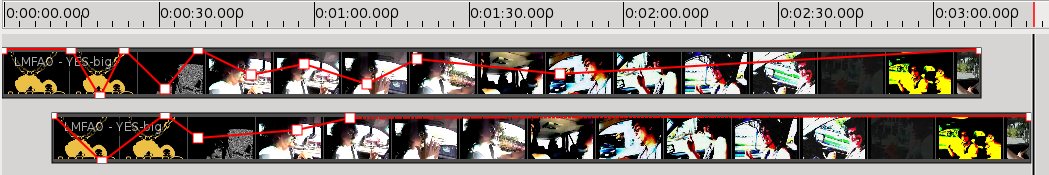
\includegraphics[width=0.48\textwidth]{images/keyframecurves}

    \end{center}

   \vspace{-30pt} \caption{Les keyframes} \vspace{-10pt} \label{Yes}

\end{wrapfigure}

\paragraph{Les keyframes}

Les keyframes définissent le début et la fin d'une animation, en
particulier dans le cadre d'effet, de texte en mouvement au dessus d'une
vidéo (dans le cadre de titres, sous-titres).

\paragraph{Speed control et time remapping}

Le speed control permet de modifier la vitesse de lecture d'un clip
dans la timeline (ralentir ou accélérer). Le time remapping est une
technique avancée de speed control, et permet de changer la vitesse de
lecture d'une partie de clip, et ainsi d' accélérer ou de ralentir des
parties d'un même clip. Cette technique est couplée aux keyframes afin
d'obtenir le résultat souhaité.

\paragraph{Gestion des Footages}

Un logiciel d'édition vidéo doit permettre d'importer les Footages
\index{Footages} à partir desquels on veut faire le montage, c'est
à dire les fichiers vidéos, audios, et images avec lesquels on
travaille. Il doit être possible de prévisualiser ces clips.

\subsection{Definition du concept d'édition timeline}

\paragraph{}

La timeline est la partie de l'interface dans laquelle on va disposer
les différents clips. Il s'agit du concept de base de l'édition vidéo
non linéaire.  Dans le cadre de l'édition timeline quelques fonctions
sont absolument indispensables, et il est nécessaire de comprendre ces
différents concepts pour comprendre la suite de ce document:

\paragraph{Découpages des clips}

\begin{wrapfigure}{r}{0.6\textwidth}

  \vspace{-20pt} \begin{center}

    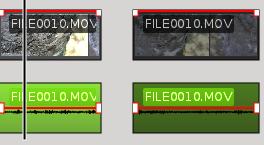
\includegraphics[width=0.38\textwidth]{images/splited}

  \end{center} \vspace{-20pt} \caption{Spliting} \label{Yes}

  \vspace{-10pt}

\end{wrapfigure}

La technique du decoupage de clip permet de diviser un Footage en
plusieurs parties afin de pouvoir les utiliser de manière indépendante.

\paragraph{}

\paragraph{Unlinking de la piste audio et de la piste vidéo}

\begin{wrapfigure}{r}{0.6\textwidth}

  \vspace{-20pt} \begin{center}

  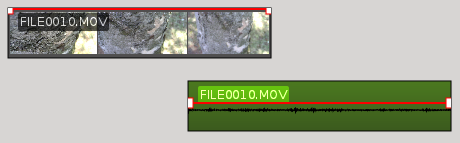
\includegraphics[width=0.38\textwidth]{images/unlinked}

  \end{center} \vspace{-30pt} \caption{Unlinking} \label{Yes}

  \vspace{-10pt}

\end{wrapfigure}

Le fait de ``de-lier'' les clips permet de gérer de manière
désynchronisée le son et la video.

\paragraph{Gestion des "in point" et  "out point" des clips}

  Permet de définir la partie d'un Footage à utiliser dans le montage
  final. Cela permet donc de redéfinir la longueur d'un clip dans la
  timeline, en ne jouant pas le début ou la fin de celui-ci.

\paragraph{}

\paragraph{Notion de layer}

\begin{wrapfigure}{r}{0.6\textwidth}

  \begin{center}

    \vspace{-20pt} 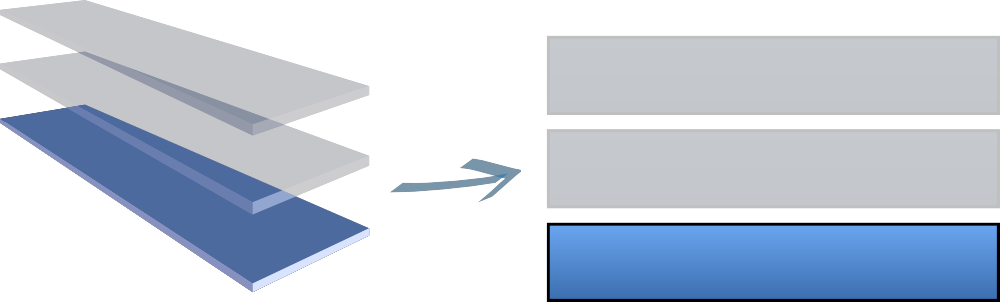
\includegraphics[width=0.38\textwidth]{images/layers}

  \end{center} \vspace{-20pt} \caption{Les layers} \label{Yes}

\end{wrapfigure}

La notion de layer est essentielle dans l'édition video avancée dans
la timeline : mixer plusieurs sources et ajouter des titres dépend de
cette fonctionnalité. Afin de comprendre, il est plus simple de faire
la comparaison avec de la peinture sur verre : on superpose plusieurs
vitres les unes au dessus des autres, chacune de ces vitres représentant
un layer. C'est la superposition des dessins de chacune des plaques
qui va nous révéler le résultat final. De plus, il existe dans les
layers une notion d'opacité , ce qui permet d'atténuer ou de révéler
intégralement les dessins des plaques inférieures.

\newpage\section{Définition du marché par segment}

\paragraph{}

Dans un premier temps, nous allons définir et analyser les différents
formats de productions audiovisuelles professionnelles. Nous avons
interviewé un certain nombre de monteurs professionnels, afin de lister
leurs besoins, (annexes 1) et en essayant de couvrir le maximum de champs
de l'édition vidéo. Nous avons pu récolter des informations provenant
de monteurs de clips vidéos, de courts métrages, de publicités,
de documentaires, de séries télévisés, et de reportages.

\paragraph{}

La littérature dans la matière (en particulier
\cite{WorldVideoNonlinearEditingMarket}) nous propose de faire une nette
distinction entre les deux segments du marché que sont:

\begin{itemize} \setlength{\itemsep}{2mm}

  \item {le monde du contenu post-produit: il s'agit de contenu dont la
    qualité de montage final est très importante. Celui-ci peut être de
    courte durée, tels que les clips vidéos ou publicités, ou bien de
    longue durée, tels que les films ou les séries télévisées. Mais
    il faut toutefois faire une différence entre ces derniers puisque
    la qualité du rendu final des films implique d'autres standards en
    terme de montage}

  \item {le monde de la production diffusée: il s'agit du contenu
    retransmis à la fois, sur internet, et sur les chaînes de
    télévisions et dont la création et la retransmission rapide
    impliquent des moyens spéciaux qui permettent de créer et
    retransmettre le contenu dans un temps restreint, voir en direct.}

\end{itemize}

\paragraph{}

Certes les deux mondes ont des contenus différents, mais surtout
ils ont des contraintes différentes, ce qui implique des divergences
importantes en terme de besoin de fonctionnalités. Nous allons donc
nous intéresser à ces deux domaines et découper notre analyse à
partir de cette distinction. Tout d'abord, nous nous intéresserons aux
fonctionnalités logicielles nécessaires à la production de contenu
post-produit. Nous analyserons ensuite les besoins intrinsèques à la
production de contenu visant le monde de la vidéo diffusée. Puis nous
essayerons de voir où se situe la frontière entre ces deux mondes afin
d'évaluer l'investissement pour les logiciels de montage vidéo libres
nécessaire pour répondre à ces marchés.

\paragraph{Le monde du contenu post-produit}

\subparagraph{}

Le monde du contenu post produit est assez vaste et au premier abord
il peut apparaître comme étant tout le contenu qui n'est pas diffusé
instantanément. Dans les faits, la distinction est plus complexe, et il
s'agit d'œuvres audiovisuelles dont le temps de post production n'est
pas un critère de première d'importance pour le choix des moyens mis
en place sur ce sujet.

\subparagraph{}

De ce fait, les formats suivants peuvent être considérés comme étant
post produits:

\paragraph{Les courts métrages}

\subparagraph{}

Les courts métrages concentrent une histoire en moins de 35 minutes. Ils
sont donc soumis à des contraintes importantes. Ils répondent à
une exigence de concision et il est donc intéressant de se poser la
question pour savoir si dans ce genre d'œuvre les monteurs utilisent
des techniques qui permettent de les rendre plus dynamiques et si des
fonctionnalités spéciales sont utilisées dans ce but.

\subparagraph{}

Dans la production de ce type d'œuvre, les interviews nous ont révélé
des fonctionnalités indispensables telles que:

\begin{itemize} \setlength{\itemsep}{2mm}

  \item{Transition (fading en priorité)}

  \item{Effets basiques (par exemple le passage en noir et blanc)}

  \item{Time remapping}

  \item{Retouche des couleurs}

  \item{Création et ajout de génériques}

\end{itemize}

\paragraph {Les publicités}

\subparagraph{}

La publicité peut s'apparenter au court métrage puisqu'il s'agit de
création courte et généralement dynamique mais dont l'objectif est
différent.  Pour atteindre cet objectif (attirer des consommateurs),
les monteurs utilisent des techniques spéciales mais les fonctionnalités
du logiciel nécessaires restent identiques à celles du court métrage.

\subparagraph{}

En revanche, la qualité du rendu est très importante: ainsi des
logiciels spécialisés sont fréquemment utilisés afin de créer le
contenu (audio, effets, images\ldots).

\paragraph {Les clips vidéos}

\subparagraph{}

Le clip vidéo est un contenu visuel qui a pour but d'illustrer une
musique. Ce type de vidéos utilise souvent beaucoup d'effets spéciaux,
et demande à priori une très grande précision au niveau de la
synchronisation entre le son et l'image. La track audio dans de telle
production sera de préférence effectuée avec un logiciel dédié à
cet effet. Pour résumer, les fonctionnalités nécessaires sont:

\begin{itemize} \setlength{\itemsep}{2mm}

  \item{Création de titres complexes (Titre en mouvement, etc\ldots)}

  \item{Ajout de titres}

  \item{Ajout d'effets}

  \item{Utilisation avancé des keyframes}

  \item{Time remapping}

\end{itemize}

\paragraph {Les films}

\subparagraph{}

La production cinématographique bénéficie de budgets beaucoup plus
élevés. Les techniques employés dans le cadre de la post production
sont plus complexes et permettent de gérer avec soin la qualité
du rendu.

\subparagraph{}

Il n'a pas été possible d'interviewer de monteur de film jusqu'à
maintenant, mais le livre ``The technique of film and video editing,
History, Theory, and Practice'' \cite{TheTechniqueOfFilmAndVideoEditing}
est un bon point de départ pour comprendre le montage cinématographique
et la très grande influence qu'il a sur les autres types de productions
audiovisuelles. On peut considérer le film comme étant une oeuvre
audiovisuelle par excellence.

\subparagraph{}

Dans le monde du cinéma, le logiciel de montage vidéo est l'un des
logiciels parmi un système connecté de logiciel de post production. Des
spécialistes de différents domaines créent les parties du film,
et le monteur a pour mission de lier tout ces éléments au travers du
logiciel de montage. Les logiciels de post production sont entre autres:

\begin{itemize} \setlength{\itemsep}{2mm}

  \item{Éditeur de son}

  \item{Création d'effet}

  \item{Retouche d'image}

  \item{Création d'animation}

  \item{\ldots}

\end{itemize}

\subparagraph{}

Les logiciels à visée professionnelle ne sont donc pas forcément
utilisables dans le monde de la création cinématographique. Il
conviendra de faire une réelle différence entre ces deux univers du
montage vidéo.

\subparagraph{}

Le logiciel de montage vidéo à proprement parler ne nécessite pas
vraiment de fonctionnalités très évoluée.  Mais la caractéristique
principal auquel doit répondre les logiciels dans ce domaine est la
possibilité d'organiser de manière efficace une très grande quantité
de footages.

Les autres logiciels de post production sont bien évidemment aussi
nécessaires afin de permettre de faire le montage de films. Ce document
n'a pas pour but de détailler ces autres logiciels.

\subparagraph{}

Une autre caractéristique de la production cinématographique, qui est
une conséquence directe de l'impératif de qualité irréprochable,
réside dans le fait que les logiciels de montage doivent permettre de
visualiser chaque image du film de manière très précise (le montage
de film se fait dans certain cas en choisissant chaque image depuis un
tableau de frames \index{frame}).


\subparagraph{}

Bien que ne demandant pas vraiment de fonctionnalités très avancées,
la création de film a des besoins assez évoluées en ce qui concerne
le logiciel de montage:

\begin{itemize} \setlength{\itemsep}{2mm}

  \item{Organisation très avancée des Footages}

  \item{Création et ajout de générique}

  \item{Passerelles avec le reste des logiciels de post production}

  \item{Preview de chaque frame dans le détail}

\end{itemize}

%TODO essayer de trouver des monteurs de films!

\newpage\paragraph {Les séries télévisées}

\paragraph{}

Le niveau de qualité des séries télévisées n'étant pas aussi élevé
que pour le montage des films, les traitements sont la plupart du temps
réalisés directement dans le logiciel de montage même. Cela implique
un nombre de fonctionnalités plus important nécessairement les fonctionnalités
suivantes:

\begin{itemize} \setlength{\itemsep}{2mm}

  \item{Création et ajout de titre}

  \item{Création et ajout de générique}

  \item{Retouche des couleurs}

\end{itemize}

\paragraph {Les documentaires}

\paragraph{}

Le documentaire est assez sobre en terme de montage. Il
réside en général dans le logiciel de montage, mais ne demande pas
de fonctionnalités spéciales. Les fonctionnalités utilisées pour
produire ce type d'œuvre sont:

\begin{itemize} \setlength{\itemsep}{2mm}

  \item{Création et ajout de titre}

  \item{Création et ajout de génériques}

  \item{Retouche des couleurs}

  \item{Utilisation des keyframes}

  \item{Transition smpte\glossary{name={smpte}, description={Society of
    Motion Picture and Television Engineers, est une association
    internationale, située aux É.-U., et composée d'ingénieurs. Elle
    développe des standards vidéos (elle en a déjà plus de 400 à
    son actif), qui sont utilisés par exemple par la télévision, ou le
    cinéma numérique (Source: http://fr.wikipedia.org/)}} \index{SMPTE}}

\end{itemize}

\newpage\paragraph{Le monde du contenu diffusé}

\paragraph{}

La plupart du contenu post produit est par la suite diffusé, la
différence que l'on fait ici entre ces deux types de production
réside dans le temps de la post production.  Dans le cas des journaux
télévisés, émission de télé, la post production est soit totalement
inexistante (dans le cas du direct), soit très courte, dans le cadre
de reportages, jeux télévisés et autres types de production visant
spécifiquement la télévision.

\paragraph {Les émissions télévisées}

\paragraph{}

Suivant leur mode de production, les émissions de télévision peuvent
être classées soit dans le contenu post-produit soit dans le contenu
diffusé. Elles sont en général diffusées très rapidement après la
création du contenu (si ce n'est en direct) et c'est la raison pour
laquelle nous les considérons comme du contenu diffusé. De plus le
fait qu'elles soient produites exclusivement pour la diffusion (aucune
commercialisation matérielle n'en est faite), cette classification
paraît naturelle.

Du fait de leur temps de production très réduit, les principales
fonctionnalités en terme de logiciel de montage sont:

\begin{itemize} \setlength{\itemsep}{2mm}

  \item{Fonctionnalité de Template qui permet d'avoir un cadre général
    de montage des présentations, en temps et ainsi faire le montage
    en direct}

  \item{Titres}

\end{itemize}

\paragraph{}

Bien évidemment, dans le cadre de la création de Templates,
les transitions ``smpte''\index{SMPTE} et les effets simples sont
généralement utilisés. Mais il n'est pas rare que les Templates à
proprement parler ne soient pas créés dans le logiciel de montage,
mais plutôt dans d'autres logiciels de création de contenu audiovisuel.

\paragraph {Évènements spéciaux (sportif, d'actualité\ldots)}

\paragraph{}

En principe ce type de production audiovisuelle n'est pas post-produit. Il
s'agit de production instantanée, et pour ce type de contenu, l'outil
de montage non linéaire doit permettre de donner une impression de
contenu post-produit alors qu'il n'en est rien. Les fonctionnalités
nécessaires sont assez similaires à celles dont on aurait besoin pour
produire des émissions de télévision.

\subparagraph{}

De plus, l'acquisition étant aussi faite en direct, il doit être possible
d'intégrer le logiciel du montage dans le système de capture d'image
et de son.

De même que pour les émissions de télévision, les Template sont
généralement produits avec des logiciels dédiés à cet effet.

\subsection{Analyse des fonctionnalités communes}

\paragraph{}

On s'aperçoit donc que de nombreuses fonctionnalités sont communes aux
différents types d'œuvres. Il convient de détailler chacune de ces
fonctionnalités afin de nous rendre compte de ce qu'elles impliquent
en terme de logiciel de montage.

\paragraph{Création et ajout de titre}

\paragraph{}

Cette fonctionnalité est utilisée dans la création de plusieurs types
de contenu:

\begin{itemize} \setlength{\itemsep}{2mm}

  \item {Séries télévisés}

  \item {Documentaires}

  \item {Clips vidéos}

\end{itemize}

\paragraph{}

Bien que cette fonctionnalité soit utilisée dans différents types de
contenu, le logiciel sera le résultat de différents paramètres. Par
exemple, dans une série télévisée le travail sur les titres sera
assez limité: on aura souvent une vidéo en arrière-plan et un titre
qui fera un fondu arrière. En revanche dans le cadre de clips vidéo,
on verra fréquemment le titre en mouvement sur le rythme de la musique
par exemple. Il est nécessaire de tout mettre en oeuvre pour répondre
à la diversité de ces besoins mais il sera plus difficile aussi bien
en terme de backend qu'en terme d'interface utilisateur de répondre
aux besoins les plus spécifiques.

\paragraph{Création et ajout de générique}

\paragraph{}

La création de générique est une fonctionnalité indispensable
à laquelle de nombreux monteurs (en particulier professionnels)
font appel. Cette fonctionnalité en terme de backend est similaire à
celle des titres puisqu'il s'agit ni plus ni moins d'ajouter du texte
au dessus d'un fond, qu'il soit animé ou non. Mais en terme d'interface
utilisateur \glossary{name={Interface Utilisateur}, description={User
Interface, il s'agit du terme  très largement employé pour définir
l'interface utilisateur, en général graphique ou GUI}} il s'agit
de deux fonctionnalités différentes puisque, par définition, le
générique est un texte qui défile dans une très grande majorité
des cas, de haut en bas.

\paragraph{}

Cette fonctionnalité est l'une des plus basiques si l'on veut
répondre aux besoins des professionnels. Elle est utilisée dans la
plupart des créations vidéo et doit être à priori standardisée et
simple à utiliser dans l'interface utilisateur afin que la mise en place
des génériques (déjà écrits) soit effectuée de manière simple et
rapide par les monteurs.

\paragraph{Gestion des Keyframes:}

\paragraph{}

Les keyframes sont utilisées dans bien des domaines, mais dans beaucoup
de cas, elles sont utilisées avec parcimonie. Elles permettent dans une
vidéo, d'animer les propriétés d'éléments ajoutés par le monteur
(effets, texte, etc\ldots). Il apparaît donc nécessaire d'avoir une
gestion minimale des keyframes, en particulier pour une gestion fine
des couleurs, mais leur utilisation est rarement vraiment avancée.

\paragraph{}

Dans la création de clips en particulier, afin de dynamiser la vidéo,
les monteurs utilisent de manière intensive les keyframes.

\subsection{Fonctionnalités spécifiques} %

Dans les faits, les fonctionnalités utilisées sont assez similaires
bien que les œuvres finales soient totalement différentes.

\paragraph{}

Quelques fonctionnalités sont apparues comme vraiment propres à la
création d'un type d'oeuvre en particulier.

\paragraph{Visualisation image par image:}

\begin{wrapfigure}{r}{0.5\textwidth}

    \begin{center}

      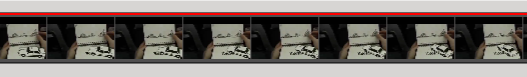
\includegraphics[width=0.48\textwidth]{images/frameByFrame}

    \end{center} \caption{Visualisation frame par frame} \label{Yes}

\end{wrapfigure}

\paragraph{}

Dans le cadre de la création de film, la prévisualisation de
chaque frame de manière précise semble être une fonctionnalité
essentielle. Cela signifie que le logiciel de montage doit permettre
de voir de manière simple chaque frame des vidéos présentes dans
la timeline. Cette fonctionnalité est aussi utile dans le cadre de la
création d'autres oeuvres, mais elle est indispensable dans le cas de
films, permettant ainsi de s'assurer de la qualité du résultat. En
effet, lors de la création d'un film, chaque frame doit être
contrôlée. Dans d'autres types d'œuvres, les exigences et les moyens
étant moins élevées, une telle fonctionnalité n'est pas indispensable.

\paragraph{Gestion avancée des Footages}

\paragraph{}

Dans le cadre de productions longues, un des problèmes auquel doit
répondre de manière satisfaisante le logiciel d'édition est la gestion
et la classification des Footages. C'est particulièrement vrai pour
les films et les séries télévisées. Dans ces types de productions
le nombre d'heures de Footages peut être très grand, et le monteur
doit dans un premier temps établir une classification des Footages. Le
logiciel de montage doit, pour répondre aux besoins des monteurs,
permettre de les ordonner de manière précise et bien pensée.

\paragraph{Intégration dans un écosystème de logiciel de post
production}

\paragraph{}

On constate, plus particulièrement dans le cadre de création de film, que le
logiciel de montage doit s'intégrer dans l'écosystème de logiciel
de post production. C'est généralement possible si ce logiciel
de montage respecte les quelques standards de la post production
d'œuvres audiovisuelles comme par exemple le Material eXchange Format
\glossary{name = {MXF}, description={Material eXchange Format ou MXF est
un conteneur utilisé par les professionnels pour les données audio et
vidéo numériques. Il s'agit d'un format défini par des standards de
la SMPTE\index{SMPTE}. (Source: wikipedia)}} \index{MXF}

\paragraph{Time remapping}

\paragraph{}

Le time remapping, comme précédemment indiqué, est particulièrement
utilisé dans la création de contenu court. Il permet d'accélérer,
où ralentir une partie d'un clip pour le rendre l'œuvre la plus
dynamique possible.

\paragraph{Gestion des Templates}

\paragraph{ }

La création de contenu non post produit demande des fonctionnalités
particulières. La fonctionnalité qui apparaît comme clé pour répondre
aux besoins liés à ce type de produit est la création de Template. Par
exemple la création de journaux télévisés ou autres évènements
sportifs demande une gestion avancée de ``moule``, ou Template, qui
permet de lier simplement les contenus des différentes caméras à un
moment donné de la retransmission.

\paragraph{ }

Cette fonctionnalité n'est pas exclusivement utilisée dans la création
de contenu en direct, mais elle est très largement utilisée dans tout
ce qui est contenu destiné à la télévision.

\paragraph{} \paragraph{}

En conclusion, on a constaté que le champ de fonctionnalité est vaste,
la plupart de ces fonctionnalités sont génériques et leur utilisation
est,par conséquent, commune à différents types d'œuvres.En revanche
ce qui varie particulièrement  est la finesse d'implémentation et le
niveau d'utilisation qu'en fait le monteur.

\newpage \section{Comparaison des principaux logiciels présents sur le
marché de l'édition vidéo professionnelle, et analyse des manques et
risques du marché}

\paragraph{}

Il conviendra d'analyser précisément les logiciels existants, qu'ils
soient propriétaires ou libres. Cette partie a pour but de rendre compte
de l'état actuel du marché des logiciels d'édition vidéo destinés
principalement aux professionnels. Cette étude portant principalement
sur les logiciels libres, ceux-ci seront évidemment inclus dans cette
analyse même si on considère que pour certains leur manque de maturité
ne leur confère pas le droit d'y figurer.

\paragraph{}

Dans cette optique, nous analyserons les points clés des logiciels.
Tout d'abord nous comparerons les fonctionnalités des logiciels, la manière
dont elles sont gérées, et nous recueillerons l'avis de professionnels
sur ces fonctionnalités et leur implémentation dans les différents
logiciels. Ensuite nous regarderons le prix de ces logiciels, nous verrons en quoi
cela peut être un argument de poids pour les logiciels libres et leur
éventuelle prise de part de marché. Nous nous concentrerons enfin
sur la documentation, livres et autres tutoriels disponibles pour ces
différents logiciels, et nous verrons quels supports sont offerts aux
professionnels pour leur utilisation.

\subsection {Historique du marché}

\paragraph{}

Les tout premiers logiciels d'édition non linéaire ont vu le jour dans
le début des années 70.  A cette époque les solutions de stockages
de données étant très limitantes, les premiers logiciels de montage
vidéo non linéaires effectivement utilisables ont vu le jour en
1989 et ceux-ci étaient basés sur les disques durs pour ce qui est du
stockage. C'est cette année là que ``Editing Machines Corp.'' et Avid
ont mis sur le marché les logiciels de montage vidéo non linéaire
ainsi que le matériel qui permettait son utilisation. Une fois de plus,
les limitations en terme de stockage de données (accès limité à
50 Gigabytes à la fois maximum), rendait l'utilisation des systèmes
de montage non linéaire inutilisables dans le domaine du cinéma,
et même dans de nombreux cas de la télévision. C'est en 1992 que
cette limitation a été surmontée: il était alors possible d'accéder
jusqu'à 7 Terabytes de données à la fois ce qui rendait envisageable
le montage de production longue de manière informatique. En
1993 Avid prend avantage de cela et s'impose comme leader mondial,
remplaçant les équipements de montage de pellicules 35mm de toutes
les principales maisons de production cinématographiques dans le
monde. Avid a été le leader incontesté du marché de l'édition
professionnel jusqu'en 2003, date à laquelle Final Cut Pro a été
considéré comme une bonne alternative à Avid par les grands acteurs
de l'édition vidéo professionnel.

\subsection{Définition des plus grands acteurs du marché}

\paragraph {Logiciels commerciaux}

\subparagraph{Avid Media Composer:}

Leader historique du marché du logiciel de montage non linéaire
professionnel. Il s'agit du produit phare de Avid Technology publié
en 1989. Depuis, ce logiciel a joué un rôle essentiel dans le
développement de ce marché.

\subparagraph{Avid Symphony:}

Evolution de Avid Media Composer, il s'agit d'une version plus complète
en terme de fonctionnalités qui a pour but de répondre aux besoins
des monteurs de productions longues tels que les documentaires et les
séries télévisées.

\subparagraph{Final Cut Pro:}

Logiciel de montage intégré dans la suite de logiciels de
post-production de Apple, Final Cut Studio. Il s'agit d'un logiciel
de montage orienté à la fois professionnel et création de film. Il
est de nos jours très utilisé et est devenu l'un des leaders mondial
du marché.

\subparagraph{Adobe Premiere Pro:}

Logiciel de montage de la suite Adobe Creative suite, il s'agit du
logiciel d'édition vidéo à visée professionnelle de Adobe System. Il
est à la fois adapté pour la création de contenu diffusé, mais aussi
de contenu post produit.

\paragraph {Logiciel en cours de libération:}

\subparagraph{Lightworks:}

Logiciel de montage actuellement commercial, très puissant, et offrant
des fonctionnalités uniques, il permet de faire parallèlement la
production diffusée et la création post-produit. Ce produit est
particulier car ses créateurs ont décidés de libérer le code source
\cite{TheLightworksOpenSourceProjectStartHere}, et ainsi  de créer une
communauté de développeurs pour en faire un projet de logiciel libre.

\paragraph {Logiciels libres:}

\subparagraph{Cinelerra:}

Logiciel de montage et de compositing libre développé principalement
par la société Héroïne \footnote{Heroine: http://heroinewarrior.com/}
et intégré par la société LMA\footnote{LMA: http://lmahd.com/}. Il
s'agit d'un logiciel de montage non linéaire avec de très nombreuses
fonctionnalités. Principalement créé pour le création de contenu
diffusé, il permet aussi de répondre aux besoins de la production
de contenu post-produit. Il s'agit du seul logiciel libre utilisé en
milieu professionnel.

\subparagraph{Kdenlive:}

Logiciel de montage libre s'intégrant dans la suite logicielle de
l'interface graphique KDE.  Ce logiciel de montage est assez complet et
peut répondre aux besoins des monteurs de contenu post-produit.

\subparagraph{PiTiVi:}

Logiciel de montage libre encore basique mais en plein développement.
Ce logiciel a pour but de répondre aux besoins du plus grand nombre,
et en particulier à ceux des professionnels de la création de contenu,
qu'il soit post produit ou non.


\subsection{Fonctionnalités}

\paragraph{}

Tout d'abord, il convient de voir quelles fonctionnalités existent
chez les différents acteurs du marché. Afin de faciliter la lecture
et avoir une vision globale de ce qui existe nous avons dessiné une
représentation sur un diagramme en toile d'araignée.  D'après les
interviews et l'analyse précédemment faite, les axes suivants ont
été choisis:

\begin{itemize} \setlength{\itemsep}{2mm}

  \item{Gestion des formats de fichiers}

  \item{Intégration dans un écosystème de post production}

  \item{Gestion des Templates}

  \item{Gestion des Footages}

  \item{Colorimétries}

  \item{Effets}

  \item{Transitions}

  \item{Support multi-platform}

\end {itemize}

\paragraph{}

Dans le schéma suivant le niveau et la qualité d'implémentation a été
prise en compte. Les retours utilisateurs ont aussi une place importante
dans cette évaluation. La plupart de ces évaluations portent sur des
données non quantifiables et c'est pour cette raison qu'aucune échelle précise
n'est donnée. Par exemple, l'ergonomie ne peut être quantifiée,
seul le ressenti des utilisateurs peut être analysé, et c'est ce
travail qui a été effectué.

\begin{figure} [H]

  \begin{center}

    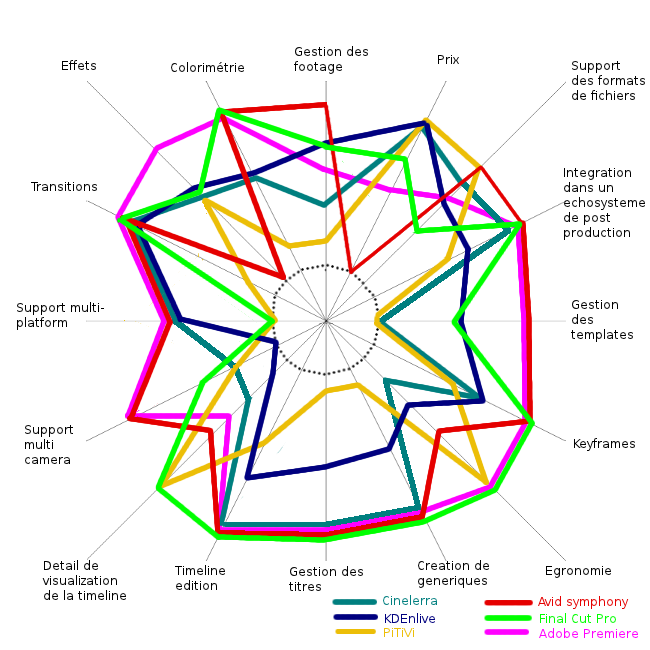
\includegraphics[width=0.9\textwidth]{images/spiderDiagramFeaturesComparision}

  \end{center}

  \caption{Comparaison des fonctionnalités des logiciels leaders sur
  le marché}

  \label{Yes}

\end{figure}

\paragraph {}

Ce schéma nous permet d'expliquer très facilement que seul le logiciel
libre Cinelerra est une place sur le marché, les lacunes de PiTiVi et
Kdenlive en terme de fonctionnalité rend leur utilisation impossible
en milieu professionnel.

\newpage

\section{Visions du marché par les professionnels du montage}

\paragraph{L'importance de la position du logiciel sur le marché}

\subparagraph{}

En ce qui concerne le choix du logiciel de montage dans une entreprise,
la connaissance que les monteurs ont du logiciel qu'ils utilisent est
essentiel.  C'est pour cela que dans de nombreux cas le premier facteur
de choix est la position de ce logiciel sur le marché de l'édition
vidéo. En effet, les différentes industries veulent avoir l'assurance qu'il
est possible de trouver de la main d'oeuvre compétente sur le logiciel
qu'elles utilisent. Mais ce n'est pas seulement la disponibilité de
personnes compétentes qui est importante, s'est également
que ces dernières puissent se former et qu'elles aient accès facilement
aux informations concernant les nouvelles résolutions des problèmes
posés par un logiciel au travers des différentes versions.

\subparagraph{}

Comme l'a souligné M. Faure lors de son interview (annexe 3), dans
son cas, il ne serait pas envisageable de changer de logiciel à moins
que le marché n'évolue. C'est à dire que l'un des critères de choix
dans son cas est la position de tel logiciel sur le marché. C'est
principalement une question de crédibilité, et donc pour éviter la
prise de risque, les professionnels préfèrent prendre la référence
du marché.

\subparagraph{}

Mais cela est principalement vrai dans les structures de taille moyenne.
Dans le cadre de petits structures, comme l'a souligné M. Veri (annexe
1) durant son interview, il serait plus logique, dans un souci de se
différencier de ses concurrents, de choisir un logiciel différent
de celui de référence. Bien évidemment ce logiciel devra répondre
convenablement à leurs besoins et permettre de satisfaire les demandes de
leurs clients. Dans son cas, M. Veri estime qu'un tel logiciel n'existe
pas et que la référence du marché (Final Cut Pro) est en réalité
la meilleure option.

\paragraph{Dépendance vis-à-vis du créateur}

\subparagraph{}

Un souci important des professionnels du montage qui ressort
des interviews est le changement de l'expérience utilisateur:
l'arrivée d'une nouvelle version est redoutée car elle demande un
temps d'adaptation pour la maitriser.  Ceci peut être illustré par
la dernière version de Final Cut Pro, qui a été très critiquée
\cite{FinalCutProXReviews}: Apple a décidé de changer le workflow
\index{workflow} des professionnels de l'édition vidéo dans la dernière
version de leur logiciel phare de ce secteur, et cela a été très mal
perçu par les professionnels. Toutefois pour M. Faure, ce problème n'est
pas trop grave, puisqu'il considère que, dans le cas où la transition
à cette nouvelle version s'avère compliquée (trop coûteuse, formation
du personnel trop onéreuse, perte de temps pour le maitriser), ils ont
toujours l'option de conserver la version courante.
Mais c'est valable seulement sur le court terme, puisqu'il n'est pas
envisageable, pour des raisons de sécurité et de support, d'utiliser
de manière commerciale un logiciel non maintenu et non supporté par
l'entreprise éditrice. Pour M. Veri en revanche, cela pose aussi un
problème important, et ayant lui même utilisé cette nouvelle version,
il considère qu'il serait préférable pour son entreprise de trouver
une autre solution.

\subparagraph{}

Dans le cadre de structures importantes, la dépendance vis-à-vis
des éditeurs est parfois considérée potentiellement dangereuse,
et donc à éviter . Par exemple, Dreamworks Picture, a décidé de
créer et de maintenir leur propre suite logiciel \cite {Dreamworks}
de post production. Leur principal objectif  est d'avoir la garantie que
leurs logiciels répondent bien à leurs besoins précis en maitrisant
leur évolution. Ils ne dépendent plus d' un éditeur externe et pour
conforter cette indépendance, cette entreprise a décidé d'utiliser
Linux comme système d'exploitation (distribution Red Hat), ce qui lui
garantit un grande liberté. De plus, la partie ``Dreamworks animations''
est cliente de la société LMA, ce qui signifie que très probablement
celle-ci utilise Cinelerra dans leur processus de post-production. De
même les sociétés de télévision française TF1 et Canal+ sont
clientes de cette même entreprise, ce qui montre bien que Cinelerra
est utilisé dans un cadre professionnel. A noter que selon M. Faure,
TF1 semble abandonner petit à petit Cinelerra au profit de Final Cut Pro.

\newpage

\section {Bilan}

\paragraph { }

Nous constatons donc que dans un marché vaste et diversifié seuls
quelques logiciels permettent à l'heure actuelle de répondre aux
besoins de la grande majorité des utilisateurs.

\paragraph{}

Les professionnels sont plutôt satisfaits des logiciels commerciaux
existants dont ils disposent avec cependant certaines limites dûs
principalement au fait que ces logiciels sont fermés et édités par une
seule entreprise (externe) . Les fonctionnalités de ces logiciels visent
à répondre à la majorité des besoins du marché, mais ils ont des
difficultés pour s'adapter à des besoins spécifiques d'entreprises .

\paragraph{}

Partant de ce constat on peut se demander si l'utilisation de logiciels
ouverts et édités par de nombreuses entreprises ne pourraient pas
prendre une place plus importante sur le marché, en offrant de nouvelles
perspectives aux acteurs du marché du montage vidéo. Les éléments
suivants peuvent être considérés comme des éléments importants sur un
marché fermé, et contrôlé par un nombre très restreint d'entreprises:

\paragraph{Plus grande autonomie vis-à-vis de la société éditrice
(développeur/designer):}

  \subparagraph{ }

    Grâce à l'utilisation de logiciel libre, il est possible de garantir
    et maintenir le logiciel en interne tout en profitant du fait que des
    personnes externes à l'entreprise, d'une part le développent, et
    d'autre part, le connaissent. Cela a pour conséquence de réduire les
    coûts d'une manière très importante tout en gardant un contrôle
    certain sur le développement du logiciel. C'est très certainement
    pour ces raisons que Dreamworks, TF1 et bien d'autres se sont mis
    à utiliser des logiciels libres.

\paragraph{Possibilité de collaboration et de communication avec les
développeurs:}

  \subparagraph{}

  Le développement des logiciels libres étant en principe fait
  publiquement, les utilisateurs (entreprises qui font le montage
  vidéos) peuvent voir l'évolution du logiciel au fur et à mesure
  de sa progression. Cela leur permet aussi de donner leur avis sur les
  directions à prendre.

\paragraph{Réduction de coût:}

\subparagraph{}

Comme l'ont souligné  M. Veri et M. Hachemi au cours de leur interview,
dans le cadre de petites structures la réduction des coûts est un
souci important.  En effet, les frais liés à l'achat de licences pour
les logiciels de montage constituent une charge financière élevée
compte tenu des prix de ces licences. L'utilisation de logiciel libre
permettrait donc, dans la très grande majorité des cas, de réduire
d'une façon significative les coûts de montage, puisque le code source
est libre d'accès.

\paragraph{Possibilité d'adaptation aux besoins précis de l'entreprise:}

\subparagraph{}

L'ouverture du code et sa mise à disposition à tous ouvre la
possibilité d'effectuer des adaptations dans le core même du logiciel
et ainsi de développer des versions spécialement adaptées aux besoins
de l'entreprise utilisatrice.

\subparagraph{}

Dans le cadre de projets commerciaux,le développement et l'adaptation de
différentes versions ne sont faites que par l'entreprise éditrice. On
peut cependant, même dans ce cadre-là, modifier, ajouter des
fonctionnalités grâce aux systèmes d'extension logicielle, mais
la flexibilité offerte par ce système reste limitée à ce que la
société éditrice veut bien mettre à disposition des développeurs
externes. (En terme d'API) \index{API} \glossary{name={API}, description={
Une interface de programmation (Application Programming Interface
ou API) est une interface fournie par un programme informatique. Elle
permet l'interaction des programmes les uns avec les autres, de manière
analogue à une interface homme-machine, qui rend possible l'interaction
entre un homme et une machine}}.

\paragraph{}

On voit que des logiciels libres sont utilisés en milieu professionnel,
mais cela reste marginal. Les opportunités que ces logiciels peuvent
apporter au monde professionnel de la post-production étant importantes,
nous allons voir comment utiliser le potentiel de ces logiciels dans
ce domaine.

\chapter{Analyse des opportunités des technologies libres dans le
domaine de l'édition vidéo et prévisions}

\minitoc \newpage

\paragraph{}

Maintenant que les besoins et que les solutions existantes ont été
analysées on rendra compte de la situation actuelle des technologies
libres et de leurs communautés. Il est aussi important de chercher les
raisons qui expliquent que ces logiciels ne sont pas utilisés par les
professionnels. Puis, nous essayerons d'envisager les solutions possibles
qui permettraient de remédier à cette situation.

\paragraph{}

Dans cette partie, nous analyserons la différence entre les manières
d'envisager la création de logiciel et nous verrons quels sont les
avantages et inconvénients de ces fonctionnements. Par la suite nous
nous concentrerons sur les frameworks existants pour faire une analyse
technique des ces technologies. Par la suite, nous analyserons les
communautés qui portent ces différents projets afin d'arriver à voir
les lacunes et les avantages de chacun des projets.  Pour finir, nous
tirerons les conclusions de cette analyse afin de trouver des solutions
aux défis qu'est la création d'un logiciel libre de montage vidéo.

\newpage

\section {Etat actuel de l'offre de logiciel libre}

Le schéma suivant permet de résumer facilement la situation:

\begin{figure} [h]
  \begin{center}
    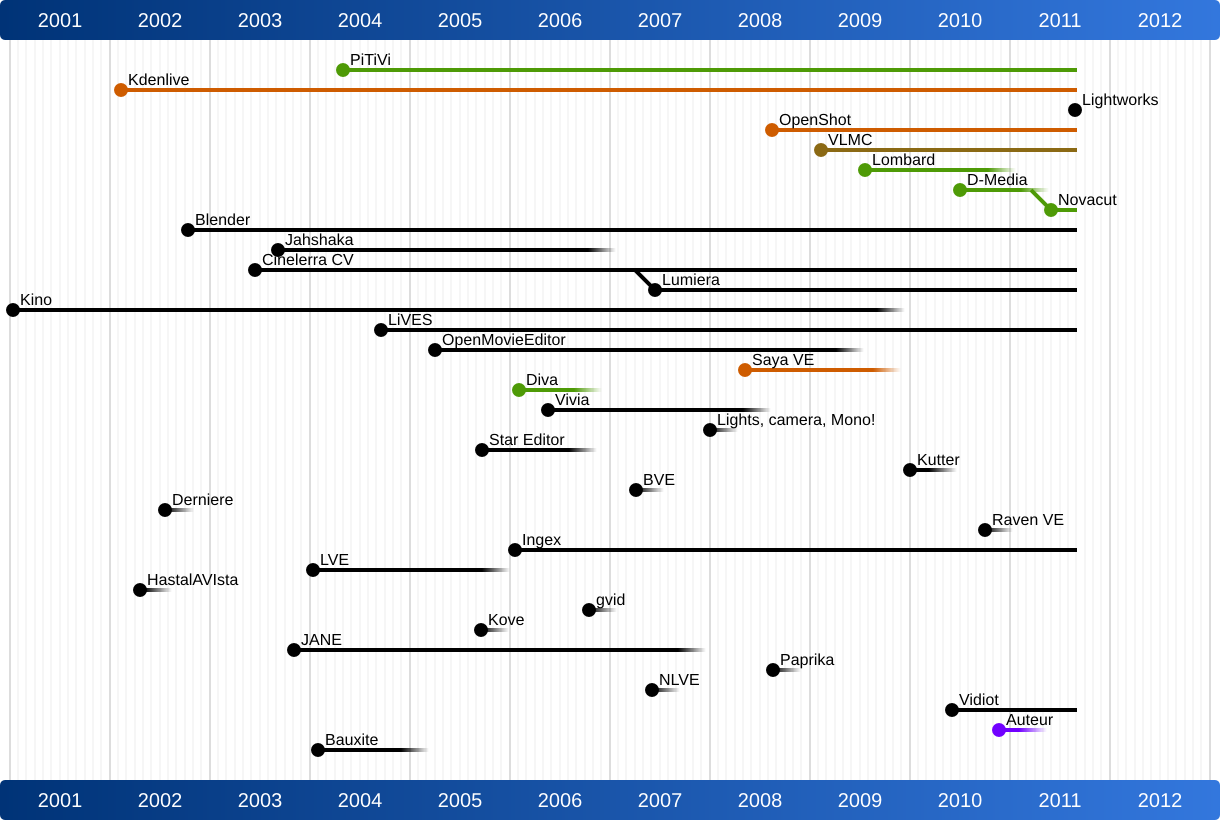
\includegraphics[width=0.9\textwidth]{images/open-source-video-editor-timeline}
  \end{center} \caption{Open source video editors timeline (Auteur:
  Jean-François Fortin, PiTiVi designer)} \label{Yes}
\end{figure}

\paragraph{ }

On constate donc que de nombreux projets de logiciel libre de montage
vidéo on vu le jours ces 10 dernières années, ayant différents
objectifs.  On peu distinguer deux types de publique visés par ces
projets:

\begin {itemize}

  \item {Les amateurs}

  \item {Les professionnels ou semi professionnels}
\end {itemize}

\paragraph {Les amateurs de montages vidéo}

\subparagraph{}

Plusieurs projets, libre permettent ou visent à répondre au besoins
des amateurs, mais à l'heure actuel même ce cas d'utilisation n'est
pas pleinement satisfait par les logiciels libres. Parmi les logiciels
ayant l'objectif de permettre de créer des montage simple on distingue:

\begin {itemize}

  \item {openshot: Logiciel avec de nombreuses fonctionnalité, mais don la
    qualité d'implémentation laisse à désirer.}

  \item {kino: Logiciel avec peu de fonctionnalité permettant de faire des
    petit montages éfficacement}

  \item {Vidiot qui vise la production de vidéo amateur simple}

\end {itemize}

\paragraph {}

Mais les logiciels ayant pour objectif de pouvoir aux besoins plus
avancés tel que ceux des professionnels (précédemment présenté
dans le cadre de la définition des plus grands acteur du marché)
peuvent être utiliser dans le cadre de montage amateur.

\paragraph{}

Un nouveau projet a aussi récemment vu le jours, ayant un but assez
différent des logiciel actuellement présent. Il s'agit de Novacut,
qui a pour but de permettre aux créateur de film et séries web de
faire le montage de manière collaborative à travers d'Internet, en
partageant les ressources (footage).

\paragraph{}

Cela montre qu'aucun projet n'a encore réussi à s'imposer et ainsi
regrouper les développeurs au sein de projets majeurs. Dans d'autre
domaine, cela a été le cas, par example dans le domaine des lecteurs
vidéo, Vlc a su surpassé ces concurrent, et ainsi supplanté le
marché des lecteur vidéo, qu'il soit libre ou non. Dans le domaine
des environnements de Bureau graphique, KDE et Gnome sont arrivés à un
stade ou leur supériorité technique, et en terme de fonctionnalités
fait d'eux des plateformes de référence.

\paragraph{}

Il est donc intéressant de se demander quel(s) technologie(s),
logiciel(s), pourrai(ent) se voir attribuer cette place dans le monde
de l'édition vidéo libre. Nous allons donc analyser les logiciel
et technologies libre les plus avancés, (précédemment mentionné
dans le cadre de l'analyse de marché: Cinelerra, Kdenlive et PiTiVi)
et ainsi voir si celui-ci, ou ceux-ci, ont le potentiel de pouvoir un
jours rivaliser avec les logiciels propriétaires sur le marché très
fermé du montage vidéo professionnels.

\paragraph{}

NB: Il aurait été intéressant d'analyser le logiciel lightworks,
en voix de libération, mais à l'heure actuel, aucun code n'a été
libéré, et par conséquent, celui-ci ne peut faire partit de cette
analyse.

\newpage

\section{Technologies}

\paragraph{}

Pour faire une analyse technique des produits permettant de faire
de l'édition vidéo, il est nécessaire d'analyser le ``core'' des
logiciels, c'est à dire la partie du logiciel où les opérations
d'édition sont effectivement réalisées. Dans ce domaines, il existe
deux façon de procéder:

\begin{itemize} \setlength{\itemsep}{2mm}

  \item{Création d'un logiciel monolithique\index{monolithique}}

  \item{Création d'un framework \glossary {name={framework},
   description={ Un framework est un ensemble d'outils et de composants
   logiciels organisés conformément à un plan d'architecture et des
   design patterns}} \index{framework}}

\end{itemize}

\subsection {Technologies monolithique\index{monolithique} VS technologies
modulaires, frameworks}


\subsubsection{Logiciels monolithiques \index{monolithique}} %FIXME Look
                                                             %for a def

\paragraph{}

Le conception monolithique \index{monolithique} dans le cadre des
logiciels d'édition vidéo, consiste à développer au sein d'un même
entité de code:

\begin{itemize} \setlength{\itemsep}{2mm}

  \item {la partie graphique et la partie de calculs
    permettant la gestion de tout ce que l'édition non linéaire
    implique}

  \item {L'interface utilisateur.}

\end {itemize}

\paragraph{}

Par le terme logiciel monolithique\index{monolithique}, il convient
de comprendre que le logiciel peut utiliser des librairies externes,
mais le core de ce même logiciel, et la logique d'édition linéaire
à proprement parler est directement faite à l'intérieur du logiciel
et non par une librairie où framework \index{framework} externe. Cela a
pour principal avantage que la conception est simplifiée pour plusieurs
raisons à savoir:

\paragraph{}

Les logiciels professionnels (commerciaux) utilisent très probablement
tous ce mode de fonctionnement (même si probablement, en interne il ont
un core qui ressemble fortement à un framework \index{framework}). Au
niveau des logiciels libres, le logiciel Cinelerra est un exemple
dans lequel les développeurs ont décidé d'utiliser ce mode de
fonctionnement.

On peu voir plusieurs conséquences immédiate de ce mode de
développement:

\begin{itemize} \setlength{\itemsep}{2mm}

  \item {Les développeurs n'ont pas la nécessité de penser
    en terme d'interface publique de programmation (API\index{API}), et
    n'ont pas à garantir la stabilité de celle-ci. Cela a pour effet que
    la qualité de l'architecture risque de ne pas être optimale puisque
    la création d'API\index{API} oblige les développeurs/architectes
    à réellement analyser les besoins de manière plus large dès le
    début de la conception. Dans le cas où l'on ne crée pas d'interface
    publique de programmation voué à être réutilisée, le risque est
    que le travail de design et d'architecture ne soit pas réalisé,
    et que le code grandisse de manière anarchique avec les différents
    développeurs qui ajoute leur morceau au fur qu'ils en ont besoin.}

  \item {Les développeurs n'ont besoin de penser l'architecture que pour
    les seuls cas d'utilisation qui sont liés à ce même logiciel,
    ils n'ont pas à voir au delà de ces use cases.}

  \item {Les erreurs en terme de design n'ont pas d'incidences aussi
    graves que dans le cas d'un framework\index{framework}.}
\end {itemize}

\paragraph{}

On se rend compte que cette manière de faire a pour principal avantage
le fait que le logiciel peut être développé plus rapidement puisque
le core du logiciel, et donc le code qui implémente la logique de
l'édition non linéaire est conçue avec pour seul cas d'utilisation,
celui du logiciel. Cependant, de nombreux inconvénients existent de
par la nature monolithique\index{monolithique} du design:

\subparagraph{Besoins en main d'oeuvre considérables:}

\subparagraph { }

Dans le cadre de logiciel d'édition vidéo, le code à produire est
considérable, comme le montre les statistiques (Annexes 2). Le logiciel
Cinelerra à lui seul fait plus d'un million de lignes. Une telle
quantité de code est difficile à maintenir et requiert des ressources
importantes en terme de main d'oeuvre. Le fait que le logiciel soit
monolithique\index{monolithique} implique que celui-ci va être utilisé
que par ce logiciel, et par conséquent, les développeurs ne peuvent
conté sur d'autre usage de ce code pour améliorer, développer le core
du logiciel.

\paragraph{Réutilisabilité:}

\subparagraph { }

L'un des inconvénients de cette manière de faire est que le code que
l'on a à l'intérieur du logiciel n'est pas réutilisable directement
par d'autres projets, et par conséquent, on peut considérer que cela
est ``individualiste``, chose qu'il convient d'éviter dans le cadre du
développement de logiciel libre afin de ne pas multiplier les efforts,
et dupliquer le code.

\paragraph{}

Cette façon de faire a été utilisée par le projet Cinelerra. Ce
logiciel est le plus avancé en terme de fonctionnalités que le
marché des logiciels libres de montage offre. On peut penser que son
architecture monolithique\index{monolithique} expliquer ce développement
plus abouti. Bien qu'il y ait évidemment de nombreux autre facteurs
tel que le fait que ce logiciel a été développé par la société
Heroine Virtual.

\subsubsection {Utilisation de  frameworks \index{framework}}

\paragraph{} L'autre possibilité est de séparer en deux parties logiciel
bien distincts l'implémentation de la logique de l'édition, lecture,
encoding vidéo (core logiciel), de la partie graphique, interaction
avec l'utilisateur final.

\paragraph {Le framework}

\subparagraph{}

La grande différence entre la conception monolithiques
\index{monolithique} et la création d'un framework \index{framework}
réside dans le le fait que dans le cadre d'un framework, on développe
une API \index{API} autour du core du logiciel. Cela résulte dans le
fait que le core est un programme (librairie) externe, réutilisable par
n'importe quel autre application.  On peut considérer que les avantages
des frameworks sont les inconvénients des applications monolithique
\index{monolithique} et vis versa. Le gros avantages des frameworks sur
une conception monolithique\index{monolithique} est la possibilité de
partager un même code à travers de multiple application. Celà permet de
réunir les efforts au travers, dans notre cas précis, de tout type d'application
multimedia.

Dans le cadre de l'édition vidéo, on peu encore distinguer deux manière
d'envisager son développement:

\begin {itemize}

  \item {Utiliser un framework multimedia généraliste, et créer les
  outils nécessaire
         au montage au dessus de celui-ci} %stupid french!\ldots On top
                                           %of it?

  \item {Créer un framework spécialement orienté montage vidéo}

\end {itemize}

Dans le monde du logiciel libre, ces deux manière d'envisager le
développement d'un framework multimedia ont été abordé par les deux
projets de framework leader sur ce segment:

\begin {itemize}

  \item {MLT qui se défini comme étant un ``Framework multimedia design
    et développé pour le brodcasting télévisé.''}

  \item {Gstreamer qui se défini comme étant un ``framework multimédia
    basé sur la notion de pipeline ce qui lui permet de nombreux types
    d'applications multimedia tel que des lecteurs multimédia, des
    logiciels de broadcasting, des logiciel de montage vidéo\ldots''}

\end {itemize}

\subparagraph {}

Au dessus de ces frameworks, deux application (interfaces graphique)
de montage vidéo se sont développé.

\begin {itemize}

  \item {PiTiVi: utilise le Framework multimedia GStreamer}

  \item {Kdenlive utilise le framework\index{framework} orienté édition et
    broadcasting MLT.}

\end {itemize}

\paragraph {}

Dans le cadre des Frameworks, nous nous intéresserons
en particulier à l'analyse de ceux-ci puisque les notions relatives
à l'édition vidéo, et la gestion de toute la partie multimédia est
réalisée par ceux-ci. Les logiciels d'édition ne sont à priori que
de simples interfaces graphiques basées sur ces frameworks, et par
conséquent leur analyse ne présente qu'un faible intérêt.

\newpage \section{Analyse technique}

\paragraph {}

Dans cette partie nous allons analyser les entrailles des trois logiciels précédemment
définis: Cinelerra, PiTiVi et Kdenlive.

\subsection{Cinelerra:}

\paragraph {}

Cinelerra est le logiciel d'édition audio et vidéo et de composition le plus
avancé dans le monde de logiciel libre. Il est développé principalement par
Adam Williams pour l'entreprise Heroine Virtual Ltd. Ce projet a été initié
en 2001 sous le nom de broadcast2000 par cette même entreprise.

\paragraph{}

Le logiciel Cinelerra a été développer principalement en C++ et est composé de 3 partie
principal interdépendantes:

\begin{itemize}

  \item{Lecture/et rendering audio vidéo}

  \item{Edition vidéo non-linéaire}

  \item{Interface graphique}

\end{itemize}

\subsubsection{Lecture et rendering}

\paragraph{}

Dans le cadre de la lecture audio et video, Cinelerra fait appelle à diverse library:

\begin{itemize}

  \item{ffmpeg: Solution compete, cross plateforme d'enregistrement, lecture, conversion
    de flux audio et vidéo. Il inclus libavcodec, librairie leader dans le domaines des codec.
    Il s'agit du core de la lecture audio et vidéo de Cinelerra.}

  \item{faac/faad: AAC audio encoder}

  \item{x264: h264 encoder}

  \item{x264: h264 encoder}

  \item{\ldots}

\end{itemize}

\subparagraph{}

Toutes ces librairies sont utilisé dans le but de lire et écrire des fichiers multimedia.
Afin de standardizer, et permettre l'utilisation de ces libraries de manière similaire
au sein du logiciel, les développeur de Cinelerra ont développé au cas par cas des pont entre
ces librairies et le reste du logiciel (Fichier dans le dossier quicktime).

\paragraph{Edition non linéaire}


\newpage \section{Analyse des communauté}

\newpage \section{Lacunes}

\newpage \section{Solutions possibles}

\newpage \chapter*{Conclusion}
\addcontentsline{toc}{chapter}{Conclusion}

\paragraph{}

Tout au long de ce document, nous avons identifié les besoins réels
des professionnels du montage vidéo. Nous nous sommes efforcés de
décrire la diversité du marché aussi bien en terme de format
de vidéo que de structures au sein de laquelle ce travail de montage
est effectué. Nous avons  cherché à connaître l'avis des
professionnels sur les outils qu'ils utilisent (grâce à des interviews),
ceci afin d'évaluer si les logiciels et les technologies "open source"
peuvent ou pourront dans le futur avoir une place dans le monde de la
production audiovisuelle professionnelle.

\paragraph{}

Au final, ce document permet de montrer que le marché du logiciel
d'édition vidéo est un marché où seules quelques entreprises
ont réussi à jouer un rôle. Nous avons aussi vérifié que les
professionnels du montage vidéo n'aiment pas changer de logiciel de
montage, et restent avec leurs habitudes tant que la maintenance est
assurée.

\paragraph{}

Nous avons pu constater que les logiciels utilisés par les professionnels
sont dans la plupart des cas (voire dans tout les cas) beaucoup plus
puissants, configurables que ce dont ils ont besoin. C'est un défaut
relevé par tous les professionnels pour tous les logiciels existants
sur le marché. Ils considèrent que leur productivité n'est pas à
son optimum essentiellement à cause de la complexité d'utilisation,
cette complexité provenant du surdimensionement en terme de nombre de
fonctionnalités de ces logiciels.

Notre analyse nous a montré qu'actuellement un seul
logiciel libre est présent sur le marché professionnel (Cinelerra),
et celui-ci se positionne sur un segment très spécifique qui est celui
des entreprises de taille importante, et des institutions publiques.

\paragraph{}

Nous avons réalisé que pour analyser le marché des logiciels
d'édition vidéo, il convient de distinguer les entreprises par leur
taille en utilisant les notions de TPE, PME et grandes entreprises. En
effet ces notions ont des conséquences directes sur les critères
de choix de logiciels.  Nous avons constaté que pour de
nombreuses  grandes entreprises, la dépendance vis-à-vis des éditeurs
de logiciels est quelque chose qu'il convient de minimiser, et ce
paramètre représente un point important dans leur choix,
et en particulier pour les logiciels de montage vidéo.
Le choix de logiciels libres permettrait de garantir cette indépendance, mais il
convient de savoir s'ils répondent aussi à toutes leurs exigences.

En ce qui concerne les entreprises de tailles moyennes, celles-ci ont pour objectif principal d'
assurer leur pérennité. Elles évitent donc de prendre des risques,
et dans le cadre du choix de logiciels de montage vidéo, elles iront
souvent vers des produits leaders sur le marché. Elles trouveront ainsi
plus facilement du personnel compétent, et auront à leur disposition
des logiciels considérés comme ``de qualité''. Dans ce cadre, les
logiciels libres ne font pas partie à l'heure actuelle des solutions
envisageables.

Les petites entreprises quant à elles recherchent des logiciels originaux et peu coûteux.
Sur ces deux points, les logiciels libres peuvent apporter de
réels avantages puisqu'ils sont tous gratuitement téléchargeables,
et librement modifiables.


\paragraph{}

Nous avons donc analysé le marché des logiciels libres sous deux points
de vues.

Premièrement d'un point de vue technique afin de comprendre ce que les
différentes technologies permettent de faire.
Nous nous sommes rendus compte qu'il n'y a pas de réelle compétition sur ce segment. Deux
technologies avec des visions différentes du problème existent. MLT
semble vouloir répondre aux problèmes posés par l'édition vidéo
et broadcasting de la manière la plus simple possible. En revanche
l'objectif de GStreamer est totalement différent car il essaie de
répondre au plus grand nombre de problèmes posés par le monde
du multimedia. Notre analyse a également mis en évidence que le logiciel
Cinelerra est techniquement très différent des autres projets: il
s'agit d'un projet important avec un code monolithique\index{monolithique}
absolument non documenté qui est maintenu par une seule entreprise et
non par une communauté.

\paragraph{}

Deuxièmement d'un point de vue des communautés afin de rendre compte
de l'état de santé des différents projets mais aussi d'analyser leurs
potentiels et leurs perspectives d'évolutions.
L'étude a mis en évidence que le projet Cinelerra est
uniquement le projet d'une entreprise (Heroine Virtual) qui vise
à répondre aux besoins d'un segment du marché de l'édition
professionnelle. L'analyse du marché nous a montré que Cinelerra
est inférieur sur de nombreux points à ses concurrents commerciaux.
Mais malgré cela, ce projet a su conquérir une partie du marché
visé. Cela montre que les avantages qu'offrent les logiciels libres
intéressent une partie du marché de l'édition video professionnelle.

Nous avons aussi vu que les communautés GStreamer et MLT sont actives,
mais compte tenu de la conception technique de ce dernier, sa communauté
est beaucoup plus petite. Ce framework permet de répondre à la plupart
des besoins des professionnels du montage et de broadcasting mais semble
limitant par sa conception dans de nombreuses situations.  Nous avons
apprécié la place prépondérante de GStreamer sur le marché des
framework multimedia. Ce logiciel est soutenu par de nombreuses entreprises
de renom. Mais nous avons également constaté que la partie montage vidéo
n'est pas actuellement le point fort de ce framework, bien que des
efforts soient faits dans ce domaine, en particulier avec la création de
la librairie gst-editing-services.

\paragraph{}

Pour conclure, les technologies de montage vidéo libres sont à l'heure
actuelle capables dans une certaines mesure de répondre aux besoins des
professionnels, mais de nombreuses limites existent toujours. Mis à part
le marché niche sur lequel Cinelerra a su se positionner, les
logiciels libres à proprement parlé ne sont actuellement pas capables
de satisfaire les professionnels, soit par leur manque d'ergonomie et
documentation, soit par leur manque de fonctionnalités.

\paragraph{}

Nous avons aussi constaté que pour concurrencer les grands acteurs du
marché, il n'est pas nécessaire de proposer une parité en terme de
nombre de fonctionnalités , les différents interviewés ont déclaré
n'utiliser que 20 à 40 pour cent des fonctionnalités proposées. Il
apparait ainsi plus important se concentrer sur les fonctionnalités
essentielles qui ont été décrites dans ce document et
faciliter le processus de montage en simplifiant l'usage du logiciel. Ceci
nous permet de penser que les logiciels libres sont potentiellement
capables de répondre à des besoins de professionnels.  Mais le manque
d'entreprises faisant la promotion, le support et la formation pour ces
logiciels est un facteur limitant.

\paragraph{}

On peut se demander si le développement actuel des logiciels libres
dans les différents domaines de l'informatique, et le soutien très
important de ce développement par de nombreuses entreprises ne vont pas
permettre à un de ces logiciels de se développer et de s'imposer dans
le milieu de l'édition vidéo.  La libération de lightworks peut jouer
un rôle sur ce marché: allons-nous voir apparaître un standard libre
de l'édition vidéo à travers ce logiciel?


\newpage
\pagestyle{empty}
\setcounter{tocdepth}{3}

\newpage

\chapter*{Annexes}
\section*{Interview de Sophian Veri,
Responsable Post Production chez Be Movie, France}

\paragraph{}
1-  Quelles logicielles d'éditions vidéos utilisez-vous à l'heure actuelle?

Sophian Veri: J'utilise exclusivement finalcut.

\paragraph{}
2- Quels formats de vidéos produisez vous?

Sophian Veri: Je produis des clips, reportages, pubs et courts métrages.

\paragraph{}
3- Ce logiciel répond-t-il à tous vos besoins en terme de montage?
Sophian Veri: généralement oui.

\paragraph{}
4- Quels défauts vous viennent à l'esprit quand vous pensez à cette outil?

Sophian Veri: le montage multicamera est mal géré, le temps de rendu trop long car le
logiciel ne fonctionne pas avec toute la mémoire vive de l'ordinateur
contrairement à la suite Adobe.

\paragraph{}
5- Considérez-vous Final Cut Pro comme étant la meilleure solution de montage,
si oui, pourquoi?

Sophian Veri: Oui, sans aucun doute. Pour sa facilité d'utilisation,
les codecs acceptés y sont nombreux et la liste des effets est
longue\ldots

\paragraph{}
6-  Quelles fonctionnalités utilisez vous au quotidien (ex: Multicamera, effets,
transitions, keyframes, time remapping, outils collaboratifs, proxy
editing, Templates...)

Sophian Veri: effets de mauvais téléviseur, time remap, cache patate (qui m'évite
de passer par after.) ralenti, fondu enchainé.

Thibault Saunier: Qu'est-ce que cache patate?
Sophian Veri: cache patate, c'est masque dans after.

\paragraph{}
7-  Quelles fonctionnalités considérez-vous comme indispensables, (même si vous
ne les utilisez pas au quotidien)?

Sophian Veri: la modification des couleurs,  tout ce qui est travail de
l'image, contraste, netteté, saturation.

\paragraph{}
8- Quel pourcentage de fonctionnalités du logiciel pensez-vous utiliser
en tout?

Sophian Veri: il y a  tellement de fonctionnalités que je serais tenté
de dire 25\%.

\paragraph{}
9- Seriez vous prêt à utiliser des logiciels ayant moins de fonctionnalités,
mais qui répondraient de manière plus efficace à vos besoins?

Sophian Veri: pourquoi pas à condition qu'ils soient aussi intuitifs et que les effets
que j'utilise soient tout aussi bien gérés.

\paragraph{}
10-  Le prix du logiciel est-il un critère de choix selon vous?

Sophian Veri: oui, en tant que nouvelle jeune entreprise, le prix est
un critère de choix.

\paragraph{}
11- Avez-vous des problèmes de stabilité (de bugs) avec finalcut?

Sophian Veri: les bugs, assez rarement.

\paragraph{}
12- La dépendance vis-à-vis du créateur du logiciel que vous utilisez
vous parait-elle être quelque chose de dangereux?

Sophian Veri: oui dans le sens où on ne sait jamais quelles transformations le
logiciel subira avec la version suivante. Il arrive que la version soit moins adaptés
et qu'elle ne me donne plus toute satisfaction. C'est le cas il me semble de Final Cut
X qui a l'air d'être raté.

\paragraph{}
13- Connaissez-vous certains logiciels libres d'édition vidéo?

Sophian Veri: Je ne sais pas vraiment ce que c'est.

Thibault Saunier: Merci bien d'avoir pris le temps de répondre

\newpage\section*{Interview de Karim Hachemi, Monteur chez Falfyprod, Film d'entreprise,
Court Métrages et film de mariage, France}

\paragraph{}
1-  Quel logiciel d'édition vidéo utilisez vous à l'heure actuel?

Karim Hachemi: Final cut mais surtout Adobe CS5.

\paragraph{}
2- Quel types de vidéo produisez vous?

Karim Hachemi: Clips, Pubs et institutionnels.

\paragraph{}
3- Ce logiciel répond-t-il à tous vos besoins en terme de montage?

Karim Hachemi: Adobe Première non, mais Final Cut oui.
Nous somme obligé d'utiliser Adobe première du fait que
le format produit par la camera Canon 5D est mal supporté par Final Cut.
Nous aurions donc besoin de les convertir et nous perderions beaucoup de
temps, c'est pourquoi nous utilisons la suite adobe bien qu'elle ne nous donne
pas complètement satisfaction.

\paragraph{}

4- Quels défauts vous viennent à l'esprit quand vous pensez à cet outil?

Karim Hachemi: Final cut est un tout petit peu plus compliqué mais
est plus complet.


\paragraph{}
5-  Quels fonctionnalités utilisez-vous au quotidien (ex: Multicamera, effets,
transitions, keyframes, time remapping, outils collaboratifs, proxy
editing, Templates...)

Karim Hachemi: Effets et transitions, en général je me sers que de ça.

\paragraph{}
6-  Quelles fonctionnalités Considérez-vous comme indispensables, (même si vous
ne les utilisez pas au quotidien)?

Karim Hachemi: le rognage de final cut sur première est mal conçu et c'est très
énervant.

\paragraph{}
7 Quel pourcentage des fonctionnalités du logiciel pensez-vous utiliser
en tout?

Karim Hachemi: Je dirais 30-35%

\paragraph{}
8- Seriez-vous prêt à utilisez des logiciels ayant moins de fonctionnalités,
mais qui répondraient de manière plus efficace à vos besoins?

Karim Hachemi: cela dépend s'il manque des fonctionnalités dont je ne me
suis jamais servi cela m'est égal.

\paragraph{}
9-  Le prix du logiciel est-il un critère de choix selon vous?

Karim Hachemi: oui.

\paragraph{}
10- Avez-vous des problèmes de stabilité (de bugs)?

Karim Hachemi: non pas trop de bugs mais ce qui est ennuyeux c'est les
rendus beaucoup trop long.

\paragraph{}
11- Connaissez-vous certains logiciels libre d'édition vidéo?

Karim Hachemi: Non, mais il faut que j'essaie.

\newpage\section*{Interview de Yves Faure, responsable technique chez TL7
(Télévision de Saint Étienne)}

\paragraph{}
1-  Quel logiciel d'édition vidéo utilisez-vous à l'heure actuelle ?

Yves Faure: Pour le montage video, j'utilise principalement Final cut pro. Il
arrive dans de très rares cas que l'on utilise adobe premiere. Notre
parc informatique est basé sur mac. En ce qui concerne l'habillage et
l'infographie on utilise ``photoshop'' et  ``After Effect'' pour les effets (bien
que dans de nombreux cas, on fasse les effets directement dans Final Cut).

\paragraph{}
2- Quel format de vidéo produisez-vous?

Yves Faure: Un peu de tout: Reportages, documentaires, plateaux magazines, films de reportage, spots
publicitaires, captations musique et théâtral.

\paragraph{}
3- Ce logiciel répond-t-il à tout vos besoins en terme de montage?

Yves Faure: Oui, largement. Nous avons des besoins spécifiques en terme d'organisation,
archivage, gestion de sous-titrage, mais cela sort du scope du logiciel de
montage.

\paragraph{}
4- Quels défauts vous viennent à l'esprit quand vous pensez à cet outil?

Yves Faure: Le problème important qui me vient à l'esprit est le fait que Final Cut 10 soit
extrêmement osé. Apple a décidé de revoir complètement l'interaction
utilisateur et cela va nous faire perdre du temps (et donc de l'argent).

Il y a aussi de petits défauts d'ergonomie qui sont irritants.

Le fait qu'il soit aussi puissant est pour nous un défaut puisque cela
complexifie la tâche du monteur.

Son prix très élevé est aussi un problème pour notre structure (bien que bien
moins cher que d'autres concurrents).

Par défaut, les fichiers de rendu video, le cache de vignette, est stocké dans
le dossier final cut pro global au  système et pas avec le projet, ce qui
signifie que l'on doit changer cela à chaque fois et une fois de plus c'est une
perte de temps importante.

Lorsqu'il y a des ruptures de timecodes dans les fichiers, le logiciel réagit mal
et cela est régulièrement une source de problème.

La gestion des formats est assez mauvaise.

Trop configurable en tout points.

Pas de sortie moniteur directe chez Apple. Pour visualiser le rendu final sur les
moniteurs et ainsi être sur de la qualité du montage (en particulier au niveau de
la lumière et des couleurs, on est obligé d'effectuer le rendu et ensuite
seulement le voir sur les moniteurs dédiés. On devrait pouvoir brancher nos Mac
sur les moniteurs et regarder en temps réel le résultat final.

\paragraph{}
5- Quelles sont les qualités apportées par ce logiciel et qui vous donne satisfaction?

Yves Faure: La dernière version de Final cut permet le réetalonage automatique (de l'image
et du son), cela va vraiment faciliter le travail des monteurs.

Le fait qu'il s'agit du standard actuel dans le milieu est très important pour
nous. Cela nous permet de communiquer facilement avec nos confrères.

Le fait aussi que l'on ait les effets directement intégrés dans le logiciel nous
permet d'accélérer le montage dans de nombreux cas.

Dans le cadre de magazines et films publicitaires, on utilise beaucoup les
animations (transformations) tel que la modification de l'échelle de l'image,
le rognage. Aussi, le lissage des bords et les ombres portés de l'image nous
permettent régulièrement de faire des montages mieux léchés.


\paragraph{}
6- Pour vous, finalcut est la meilleure solution de montage?

Yves Faure: Oui, c'est sûr.

\paragraph{}
7-  Quelles fonctionnalités utilisez-vous au quotidien (ex: Multicamera, effets,
transitions, keyframes, time remapping, outils collaboratifs, proxy
editing, Templates...)

Yves Faure: Au quotidien, nous utilisons: Transition, effet, mixage audio, montage cut,
retouche de couleurs, étalonnage, colorimétrie, multi-images, gestion de la
vitesse par clip entier, pas de time remapping à proprement parlé.

\paragraph{}
8-  Quelles fonctionnalités considérez-vous comme indispensables, (même si vous
ne les utilisez pas au quotidien)?

Yves Faure: Je pense que le multicamera (pour la couverture d'évènement tel que les
concerts) est la fonctionnalité importante, même si elle n'est pas utilisée au quotidien.

\paragraph{}
9- Quel pourcentage des fonctionnalités du logiciel pensez-vous utiliser
en tout?

Yves Faure: En général 10\%, jusqu'à 50\% maximum.

\paragraph{}
10- Seriez-vous prêt à utiliser des logiciels ayant moins de
fonctionnalités, mais qui répondrait de manière plus efficace
à vos besoins?

Yves Faure: Non, car nous sommes très attachés à la connaissance du logiciel.
Changer de logiciel signifie 40 personnes à former, changer les
habitudes et cela est très complexe en particulier pour les professionnels
du montage vidéo! Nous avons une solution qui nous convient et qui est leader
sur le marché, il faudrait une vrai évolution du marché pour que l'on pense à
changer.

\paragraph{}
11-  Le prix du logiciel est-il un critère de choix selon vous?

Yves Faure: Oui et non, c'est cher mais ça marche. Autant se donner les moyens pour avoir
un produit qui nous permet de gagner par la suite.

\paragraph{}
12- Avez-vous des problèmes de stabilité (de bugs) avec Final Cut?

Yves Faure: Non, la stabilité est un point fort de Final Cut.

\paragraph{}
13- La dépendance vis-à-vis du créateur du logiciel que vous utilisez
vous paraît-elle être quelque chose de dangereux ?

Yves Faure: Non, on s'arrange comme on peut. La version que l'on utilise actuellement
nous convient. S'il faut continuer avec celle-ci, on le fera.


\newpage
\printindex
\listoffigures

\newpage
\printglossary

\newpage
\bibliography{biblio}

\end{document}
